%waiting for a girl like you
{\color{blue}
\section{Experimental Results}\label{sec:experimental}
The objective of this experimental evaluation is to assess whether PbCRPE can achieve competitive credit risk prediction quality compared with other state-of-the-art works while simultaneously providing explainable predictions based on combinations of multiple features that jointly contribute to the prediction. The evaluation considers two complementary aspects of prediction quality, assessed using AUC and Type~II Error, two commonly used metrics in credit risk prediction that capture different aspects of predictive quality: the overall ability of the predictor to discriminate between defaulters and non-defaulters and its ability to correctly identify defaulters, respectively. While a competitive AUC indicates that PbCRPE maintains a strong overall discrimination capability, particular emphasis is placed on Type~II Error because incorrectly classifying a defaulter as a non-defaulter may result in direct financial losses for lending institutions. Therefore, achieving a low Type~II Error is particularly relevant from a practical credit risk perspective, and the experimental evaluation investigates whether PbCRPE can provide an advantage in this aspect while maintaining competitive overall prediction quality.\newline

PbCRPE is compared with twelve recent state-of-the-art credit risk prediction works using the same experimental setup and twelve public and private credit risk datasets. These works were selected from studies published between 2024 and 2025 because they represent recent developments in machine-learning-based and explainable credit risk prediction, report competitive prediction results, and evaluate their algorithms on benchmark datasets that overlap with or are comparable to those considered in this work. The results show that PbCRPE achieves competitive prediction quality in terms of AUC compared with the evaluated state-of-the-art works, while obtaining the best overall result in terms of Type~II Error. This result is particularly relevant from a practical perspective because a lower Type~II Error indicates a lower proportion of actual defaulters incorrectly classified as non-defaulters. Therefore, the experimental evaluation shows that PbCRPE maintains competitive overall prediction quality while achieving a particular advantage in identifying actual defaulters and reducing the risk of incorrectly classifying them as non-defaulters.

\subsection{Datasets}

The experimental evaluation was conducted using twelve credit risk datasets obtained from both public and private sources. The datasets were selected because they represent diverse credit risk scenarios while sharing the two characteristics addressed by the proposed PbCRPE algorithm: mixed-type data, including numerical and categorical features, and different degrees of class imbalance. The diversity in feature types and class distributions allows the prediction quality of PbCRPE to be evaluated under different data conditions.\newline

Table~\ref{conjuntodedatos} summarizes the main characteristics of the datasets, including the number of instances, number of features (total, numerical, and categorical), class distribution, imbalance ratio (IR), and data source. The eleven public datasets were obtained from the UCI Machine Learning Repository\footnote{\url{https://archive.ics.uci.edu/}} and Kaggle\footnote{\url{https://www.kaggle.com/}}, two widely used repositories for benchmarking credit risk prediction algorithms. The twelfth dataset was provided by a private financial institution. Due to a confidentiality agreement, the identity of the institution and further information about the dataset cannot be disclosed. The datasets vary substantially in both size and class distribution, ranging from 628 to 150,000 instances and from nearly balanced datasets (IR = 1.09) to highly imbalanced datasets (IR = 13.96). Consequently, the experimental evaluation covers a broad spectrum of credit risk scenarios, allowing the prediction quality of PbCRPE to be assessed under different levels of class imbalance.
	\begin{table}[H]
		\centering
		\caption{Characteristics of the twelve credit risk datasets used in the experimental evaluation.}
		\label{conjuntodedatos}
		\resizebox{12cm}{!}{%
			\begin{tabular}{lccccccc}
				\hline
				\multicolumn{1}{c}{\textbf{Dataset}} &
				\textbf{Instances} & \textbf{Features} &
				\textbf{Numerical/Categorical} &
				\textbf{No-defaulter} & \textbf{Defaulter} &
				\textbf{IR} & \textbf{Domain} \\ \hline
				AER            &   1,319   & 12 & 9/3   &   1,023  &    296  &  3.45  & Public  \\
				Australia      &     690   & 14 & 6/8   &     307  &    383  &  1.24  & Public  \\
				Japan          &     690   & 15 & 6/9   &     307  &    383  &  1.24  & Public  \\
				EIZ            &   5,510   & 22 & 13/9  &   2,295  &  3,215  &  1.40  & Private \\
				German         &   1,000   & 20 & 7/13  &     700  &    300  &  2.33  & Public  \\
				HMEQ-Data      &   3,364   & 12 & 10/2  &   3,064  &    300  & 10.21  & Public  \\
				Taiwan         &  30,000   & 24 & 20/3  &  23,364  &  6,636  &  3.52  & Public  \\ % corrected: 30,000
				GMSC           & 150,000   & 11 & 10/1  & 139,974  & 10,026  & 13.96  & Public  \\
				Heloc          &  10,459   & 23 & 23/0  &   5,000  &  5,459  &  1.09  & Public  \\
				Loan data set  &     628   & 12 & 7/4   &     332  &    296  &  1.12  & Public  \\
				PPDai          &  55,596   & 29 & 22/7  &  48,413  &  7,183  &  6.74  & Public  \\
				Thomas dataset &   1,225   & 14 & 14/0  &     902  &    323  &  2.79  & Public  \\
				\hline
		\end{tabular}}
	\end{table}
\subsection{Credit risk prediction quality}

Figures~\ref{fig:rocauc} and~\ref{fig:type2} compare the prediction quality of PbCRPE with that of the twelve selected state-of-the-art approaches using AUC and Type~II Error, respectively. For each dataset, a stratified 5-fold cross-validation procedure was employed, in which the data were divided into five folds while preserving the class distribution across folds. In each iteration, four folds (approximately 80\% of the instances) were used for training and the remaining fold (approximately 20\%) was used for testing. The process was repeated five times, with each fold serving once as the test set. The same cross-validation protocol was applied to PbCRPE and all compared approaches to ensure a fair and consistent evaluation. The reported AUC and Type~II Error values correspond to the mean results obtained across the five folds. Figure~\ref{fig:rocauc} reports the mean AUC across the twelve evaluated datasets, whereas Figure~\ref{fig:type2} presents the corresponding mean Type~II Error across the same datasets.\newline

\begin{figure}[H]
	\centering
	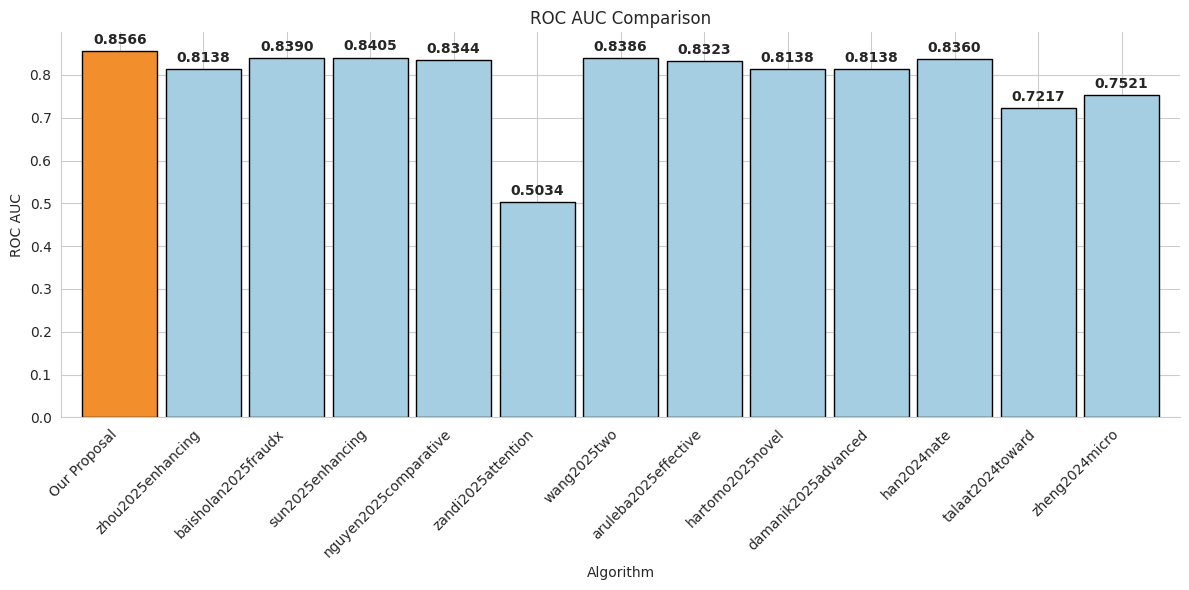
\includegraphics[width=0.9\linewidth]{img/rocauc}
	\caption{Mean AUC obtained by PbCRPE and the compared state-of-the-art approaches across the twelve evaluated credit risk datasets. Higher values indicate better prediction quality.}
	\label{fig:rocauc}
\end{figure}

\begin{figure}[H]
	\centering
	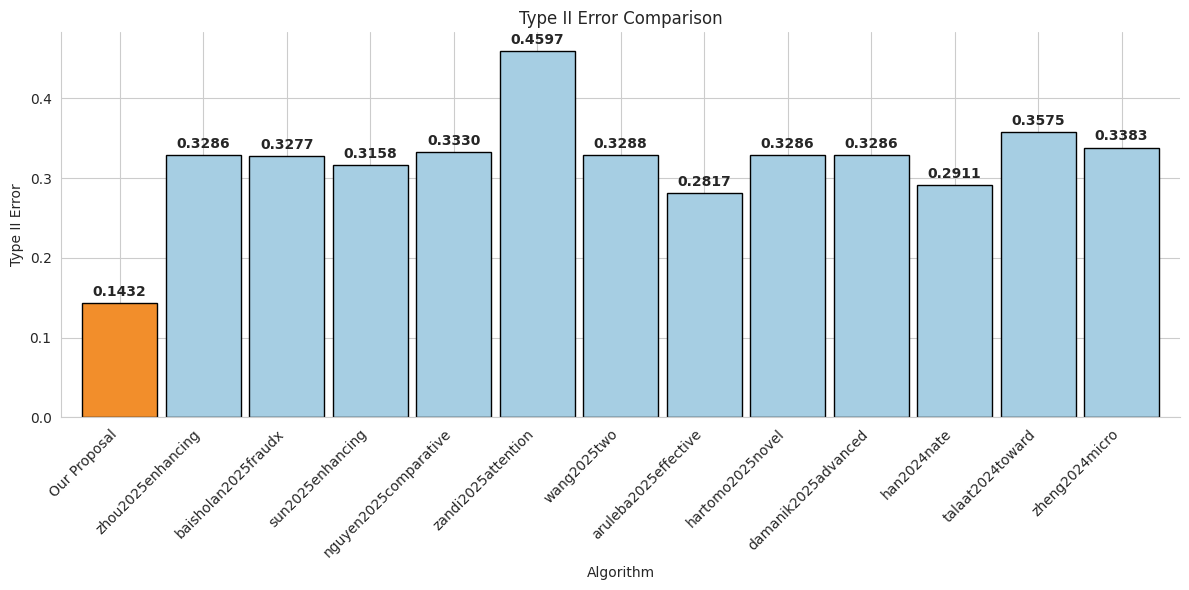
\includegraphics[width=0.95\linewidth]{img/errortipoII}
	\caption{Mean Type~II Error obtained by PbCRPE and the compared state-of-the-art approaches across the twelve evaluated credit risk datasets. Lower values indicate better prediction quality.}
	\label{fig:type2}
\end{figure}

Across the twelve evaluated datasets, PbCRPE achieves a mean AUC of \textbf{0.8566} and a mean Type~II Error of \textbf{0.1432}. The AUC results indicate that PbCRPE provides competitive prediction quality compared with the selected state-of-the-art approaches. In particular, PbCRPE attains the highest AUC on several datasets while maintaining competitive results on the remaining datasets. In terms of Type~II Error, PbCRPE achieves the best overall result among the evaluated approaches, indicating a lower proportion of actual defaulters incorrectly classified as non-defaulters.\newline

To further assess the statistical significance of the observed differences, the Friedman test was applied separately to the AUC and Type~II Error results across the twelve evaluated datasets. This non-parametric test evaluates whether statistically significant differences exist among the compared approaches based on their ranks across datasets. For both metrics, the best-performing approach within each dataset was assigned rank~1, with higher rank values corresponding to lower prediction quality. Consequently, lower average ranks indicate better overall prediction quality across the evaluated datasets. The corresponding Friedman test results are presented in Figures~\ref{fig:friedman_auc} and~\ref{fig:friedman_type2}.

\begin{figure}[H]
	\centering
	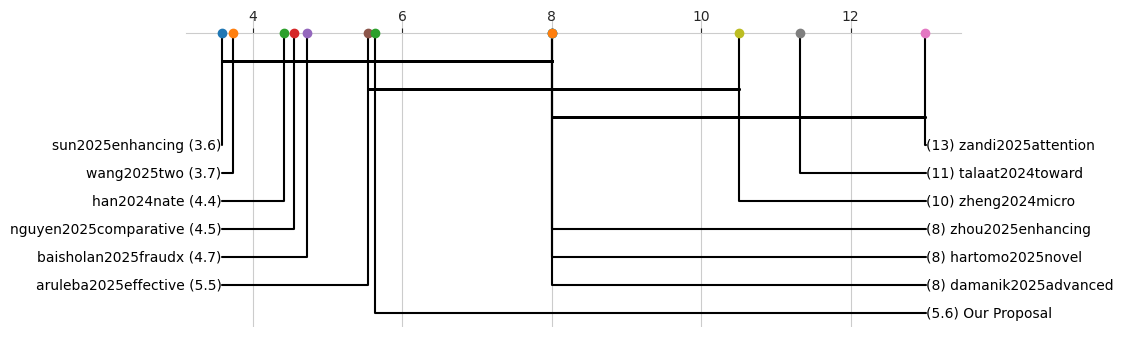
\includegraphics[width=0.95\linewidth]{img/friedman_auc}
	\caption{Friedman test results for AUC across the twelve evaluated credit risk datasets.}
	\label{fig:friedman_auc}
\end{figure}

\begin{figure}[H]
	\centering
	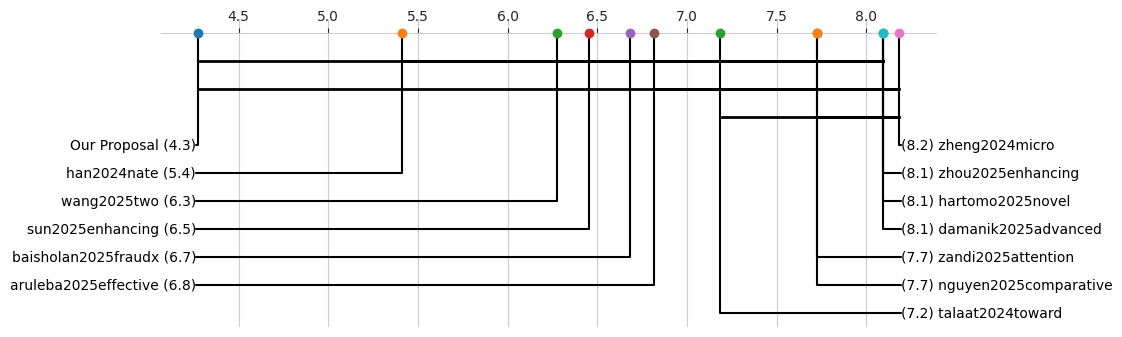
\includegraphics[width=0.95\linewidth]{img/friedman_typeiierror}
	\caption{Friedman test results for Type~II Error across the twelve evaluated credit risk datasets.}
	\label{fig:friedman_type2}
\end{figure}

For AUC, the statistical analysis indicates that PbCRPE remains competitive with the state-of-the-art works, as reflected by its relative ranking across the evaluated datasets. Although PbCRPE does not necessarily outperform all compared approaches in terms of AUC, its overall ranking demonstrates that its prediction quality is comparable to that of recent works reported in the literature.\newline

While the AUC results show that PbCRPE provides competitive prediction quality compared with the evaluated works, the Type~II Error results show that PbCRPE achieves the best overall result among the evaluated works. The proposed algorithm obtains the lowest mean Type~II Error and the best mean rank for this metric across the evaluated datasets. This result is particularly relevant from a practical credit risk perspective because Type~II Error measures the proportion of actual defaulters incorrectly classified as non-defaulters. A lower value therefore indicates a greater ability to identify customers who are likely to default, reducing the risk of incorrectly considering them as non-defaulters.\newline

To determine which pairwise differences between works are statistically significant, a Nemenyi post-hoc test was performed following the Friedman analysis. The resulting comparisons provide additional evidence regarding the relative position of PbCRPE with respect to the evaluated state-of-the-art works. For AUC, the post-hoc analysis shows that PbCRPE remains within the group of competitive works, with no statistically significant disadvantage with respect to the evaluated works. For Type~II Error, PbCRPE obtains the lowest mean rank, consistent with its lowest mean Type~II Error across the evaluated datasets. These results indicate that the proposed algorithm achieves the best overall position for this metric while maintaining competitive AUC results.\newline

From a practical perspective, the results obtained for Type~II Error are particularly important in credit risk prediction because failing to identify a defaulter may result in direct financial losses for lending institutions. Therefore, the low Type~II Error obtained by PbCRPE reflects its ability to reduce the proportion of actual defaulters incorrectly classified as non-defaulters. This result is particularly relevant because PbCRPE achieves the lowest Type~II Error while maintaining competitive overall discrimination capability in terms of AUC. Taken together, these results indicate that PbCRPE provides competitive prediction quality compared with recent state-of-the-art works while achieving the best overall results in terms of Type~II Error.


%\subsection{Explanation Analysis}\label{sec:explanation-analysis}
%The explanation analysis evaluates whether the contrast pattern mining algorithm provides sufficient pattern coverage for the instances evaluated by PbCRPE. In particular, we verify whether, for each evaluated instance $x$, at least one contrast pattern mined from a cluster associated with the predicted class covers $x$. This analysis directly evaluates the coverage assumption defined for the prediction and explanation stages. A prediction is considered covered when $\mathcal{P}*{c,j}(x) \neq \emptyset$ for at least one cluster $C*{c,j}$ associated with the predicted class $c$.\newline

%Across the twelve evaluated credit risk datasets, all evaluated instances were covered by at least one contrast pattern mined from a cluster associated with the predicted class. Consequently, the explanation stage successfully identified a covering contrast pattern for every evaluated prediction, and no fallback mechanism was required. This result provides empirical evidence that the proposed clustering and contrast pattern mining approach provides complete pattern coverage across the evaluated datasets.\newline

%Although this observation does not constitute a theoretical guarantee that every possible future instance will be covered, it confirms the empirical validity of the coverage assumption under the experimental conditions considered in this study.

\subsection{Discussion}

PbCRPE achieves competitive prediction quality compared with the twelve evaluated state-of-the-art works while simultaneously providing an explanation for each prediction. This dual capability, integrating prediction and explanation within a single algorithm, represents an important advantage over post-hoc explanation techniques such as SHAP and LIME, which typically express explanations through feature-level contribution or importance scores rather than explicitly representing a conjunction of feature-value conditions. This distinction is particularly relevant in credit risk prediction, where default risk is generally associated with combinations of financial and personal attributes rather than individual features considered in isolation~\cite{aruleba2025improved}.\newline

A key contribution of PbCRPE is therefore the representation of explanations as contrast patterns rather than as independent feature-importance scores. While SHAP assigns a contribution value to each feature according to its contribution to the prediction, and LIME estimates the local importance of features using an interpretable surrogate model, PbCRPE provides an explicit conjunction of $feature\#value$ conditions that jointly characterizes the prediction. Consequently, the explanation not only identifies which features are involved in the prediction, but also specifies the particular combination of conditions shared by the new instance and multiple similar instances within the selected cluster. For example, a pattern such as $\mathit{credit\_history} \neq \texttt{A34} \wedge \mathit{amount} < \$7{,}824 \wedge \mathit{duration} > 28\,\mathrm{months} \wedge \mathit{installment\_rate} > 2\% \wedge \mathit{num\_loans} \leq 1$ represents a joint configuration of conditions rather than a set of independent feature contributions. This representation preserves the relationships among the conditions and provides an explanation associated with a group of similar instances rather than with isolated feature contributions.\newline

This difference should not be interpreted as indicating that SHAP or LIME cannot account for feature interactions. Rather, the distinction lies in how the resulting explanation is represented. SHAP and LIME primarily summarize the local contribution or importance of individual features, whereas PbCRPE explicitly expresses the explanation as a conjunction of conditions that jointly cover the instance and are shared by similar instances. Therefore, PbCRPE provides a pattern-based representation that can be directly interpreted as a combination of $feature\#value$ conditions associated with the predicted class.\newline

To illustrate the explanation process, Table~\ref{tab:example_instance} presents an example of an instance from the German credit dataset that was classified by PbCRPE as \textit{defaulter}.\newline

\begin{table}[H]
	\centering
	\caption{Example instance from the German credit dataset.}
	\label{tab:example_instance}
	\renewcommand{\arraystretch}{1.15}
	\begin{tabularx}{\textwidth}{
			>{\raggedright\arraybackslash}p{0.19\textwidth}
			>{\centering\arraybackslash}p{0.08\textwidth}
			>{\centering\arraybackslash}p{0.12\textwidth}
			X
		}
		\toprule
		\textbf{Feature} & \textbf{Type} & \textbf{Value} & \textbf{Description} \\
		\midrule
		
		\textit{estatus\_cuenta} 
		& C 
		& A14 
		& No checking account \\
		
		\textit{duracion} 
		& N 
		& 36 
		& Duration of the credit: 36 months \\
		
		\textit{historial\_creditos} 
		& C 
		& A30 
		& No credits taken/all credits paid back duly \\
		
		\textit{finalidad} 
		& C 
		& A43 
		& Radio/television \\
		
		\textit{monto\_credito} 
		& N 
		& 3342 
		& Credit amount: \$3,342 \\
		
		\textit{cuenta\_ahorro} 
		& C 
		& A65 
		& Unknown/no savings account \\
		
		\textit{empleo\_actual} 
		& C 
		& A75 
		& Present employment for 7 years or more \\
		
		\textit{tasa\_interes} 
		& N 
		& 4 
		& Installment rate: 4\% of disposable income \\
		
		\textit{genero\_estadocivil} 
		& C 
		& A93 
		& Male, single \\
		
		\textit{aval} 
		& C 
		& A101 
		& No other debtors or guarantors \\
		
		\textit{residencia} 
		& N 
		& 2 
		& Present residence since 2 years \\
		
		\textit{propiedad} 
		& C 
		& A123 
		& Car or other property, excluding real estate and savings agreements/life insurance \\
		
		\textit{edad} 
		& N 
		& 51 
		& Age: 51 years \\
		
		\textit{planesdepago} 
		& C 
		& A143 
		& No other installment plans \\
		
		\textit{vivienda} 
		& C 
		& A152 
		& Own housing \\
		
		\textit{numero\_creditos} 
		& N 
		& 1 
		& One existing credit at this bank \\
		
		\textit{empleo} 
		& C 
		& A173 
		& Skilled employee/official \\
		
		\textit{dependientes} 
		& N 
		& 1 
		& One person liable to receive maintenance \\
		
		\textit{telefono} 
		& C 
		& A192 
		& Telephone registered under the customer's name \\
		
		\textit{trabajo\_extranjero} 
		& C 
		& A201 
		& Foreign worker: yes \\
		
		\bottomrule
	\end{tabularx}
\end{table}

For the instance shown in Table~\ref{tab:example_instance}, PbCRPE first considers the clusters associated with the predicted class. Using the contrast pattern-based similarity score defined in Equation~\ref{eq:cluster_similarity}, the cluster with the highest similarity to the new instance is selected. Subsequently, among the contrast patterns from the selected cluster that cover the new instance, the pattern with the highest support is selected according to the criterion defined in Equation~\ref{eq:pattern_selection}:

\[
\begin{aligned}
	&\mathit{credit\_history} \neq \texttt{A34} \wedge
	\mathit{amount} < \$7{,}824 \wedge
	\mathit{duration} > 28\,\mathrm{months} \\
	&\wedge\ 
	\mathit{installment\_rate} > 2\% \wedge
	\mathit{num\_loans} \leq 1
\end{aligned}
\]

Thus, the selected contrast pattern covers the instance because all of its $feature\#value$ conditions are simultaneously satisfied. For example, the condition $\mathit{credit\_history} \neq \texttt{A34}$ is satisfied because the instance has an \textit{No credits taken/all credits paid back duly} credit history, which corresponds to a value different from \texttt{A34}. Similarly, $\mathit{amount} < \$7{,}824$ is satisfied because the credit amount is \$3,342; $\mathit{duration} > 28\,\mathrm{months}$ is satisfied because the duration is 36 months; $\mathit{installment\_rate} > 2\%$ is satisfied because the installment rate is 4\%; and $\mathit{num\_loans} \leq 1$ is satisfied because the instance has one existing loan. Since a contrast pattern is defined as a conjunction of conditions, all these conditions must be satisfied simultaneously for the pattern to cover the instance. Importantly, the pattern is not interpreted as a collection of independent feature contributions. Rather, its conjunction represents a combination of $feature\#value$ conditions shared by the new instance and multiple similar instances within the selected cluster. Consequently, the contrast pattern provides a concise representation of the combination of conditions associated with the predicted credit risk class.\newline

The example also illustrates the role of performing contrast pattern mining at the cluster level rather than directly at the class level. Instead of extracting patterns intended to represent all instances belonging to the same class, PbCRPE mines contrast patterns from groups of similar instances. This strategy allows different local structures within the same class to be captured, enabling the resulting patterns to represent $feature\#value$ conditions that are more specific to particular groups of similar instances. Therefore, the resulting explanations are associated not only with the predicted class but also with a specific group of similar instances represented by the selected cluster.\newline

The experimental results confirm that the coverage condition required by the explanation procedure was satisfied for all evaluated instances. In particular, for every evaluated instance across all twelve datasets, at least one contrast pattern mined from a cluster associated with the predicted class covered the instance. Therefore, the similarity score could be computed from covering contrast patterns for all evaluated instances, and the explanation procedure could be applied without requiring any fallback mechanism. These results provide empirical evidence that the coverage condition defined in the explanation procedure was consistently satisfied under the experimental conditions considered in this study.\newline

Taken together, these results indicate that PbCRPE combines competitive prediction quality with explanations based on contrast patterns that represent combinations of $feature\#value$ conditions shared by similar instances. By integrating prediction for mixed-type and imbalanced data with cluster-level contrast pattern mining and representative pattern selection, PbCRPE generates explanations that are directly associated with groups of similar instances rather than isolated feature contributions. These results support the applicability of the proposed algorithm to credit risk datasets involving mixed-type features and class imbalance, where both prediction quality and explainable decision support are relevant.
}